% !TeX spellcheck = en_US
% Chapter 1

%\chapter{Chapter Title Here} % Main chapter title
%
%\label{Chapter1} % For referencing the chapter elsewhere, use \ref{Chapter1} 

%----------------------------------------------------------------------------------------

% Define some commands to keep the formatting separated from the content 
\newcommand{\keyword}[1]{\textit{#1}}
\newcommand{\sm}[0]{$M_\odot$}
\newcommand{\todo}[1]{\texttt{\color{red}\#TODO: #1}}
\newcommand{\erf}[1]{\text{erf}\left(#1\right)}
%\newcommand{\option}[1]{\texttt{\itshape#1}}

%----------------------------------------------------------------------------------------

\section{Galatic setup}
	\subsection{Units}
		Computer simulations are sensitive to rounding errors due to the lack of infinite precision when representing decimal numbers. Really small numbers as well as really big ones tend to have bigger errors than those close to the unity, as can be seen on \autoref{fig: IEEE-754}.
		\begin{figure}[h]
			\centering
			\includegraphics[width=0.8\linewidth]{"../Files/Week 3/floating"}
			\caption{Floating point precision for different values, for a 32 bit and 64 bit holders.}
			\label{fig: IEEE-754}
		\end{figure}
		
		Under the International System of Units, distances are measured on meters, times on seconds, and mass on kilograms, nevertheless black holes are too heavy to be measured on kilograms, galaxies sizes too big to be quantified on meters, and time scales too large for a second. Because of that, the following units will be used throughout this document:
		\begin{table}[h]
			\centering
			\caption{Natural units}
			\label{tb: units}
			\begin{tabular}{c|c}
				\hline
				\textbf{Physical property} & \textbf{unit} \\
				\hline
				Length & 1 kilo-parsec (kpc) \\
				Mass & $10^5$ solar masses ($10^5$ \sm) \\
				Time & 1 giga-year (Gyr) \\
				\hline
			\end{tabular}
		\end{table}		
		
		\subsubsection{Universal gravitational constant}
			First quantified by Henry Cavendish the gravitational constant has a value of $G_0 = 6.67408\times10^{-11}$ on SI units of m$^3$s$^{-2}$kg$^{-1}$. With the units of length, mass and time on \autoref{tb: units}, the constant of gravity to be used is given by:
			\begin{equation}
				\small
				G = G_0 \left(\dfrac{1 \text{ kpc}^3}{\left(3.0857\times10^{19}\right)^3  \text{ m}^3}\right)\left(\dfrac{\left(3.154\times10^{16}\right)^2 \text{ s}^2}{1 \text{ Gyr}^2}\right)\left(\dfrac{1.98847\times10^{35} \text{ kg}}{10^5 M_\theta}\right) = 0.4493 \dfrac{\text{kpc$^3$}}{\text{Gy$r^210^5$\sm}}
			\end{equation}
			
		\subsubsection{Hubble constant}
		The hubble constant is frequently used as $H_0 = 67.66 \pm 0.42$ kms$^{-1}$Mpc$^{-1}$ \cite{aghanim2018planck}, stating the speed of an astronomical body on kms$^{-1}$ at a distance of 1 Mpc. Nevertheless, the hubble constant has units of 1/time, thus, taking into account the units on \autoref{tb: units} one gets:
		\begin{equation}
			H = H_0 \left(\dfrac{1 \text{ kpc}}{3.0857\times10^{16} \text{ km}}\right)\left(\dfrac{3.154\times10^{16} \text{ s}}{1 \text{ Gyr}}\right)\left(\dfrac{1 \text{ Mpc}}{1000 \text{ kpc}}\right) = 6.916\times10^{-2}\text{ Gyr$^{-1}$}
		\end{equation}
		
		
	\subsection{Mass distributions}
		The host galaxy has two mass distributions that are superimposed, one for dark matter and the other one for all the luminous or baryonic matter.
		\begin{figure}[h]
			\centering
			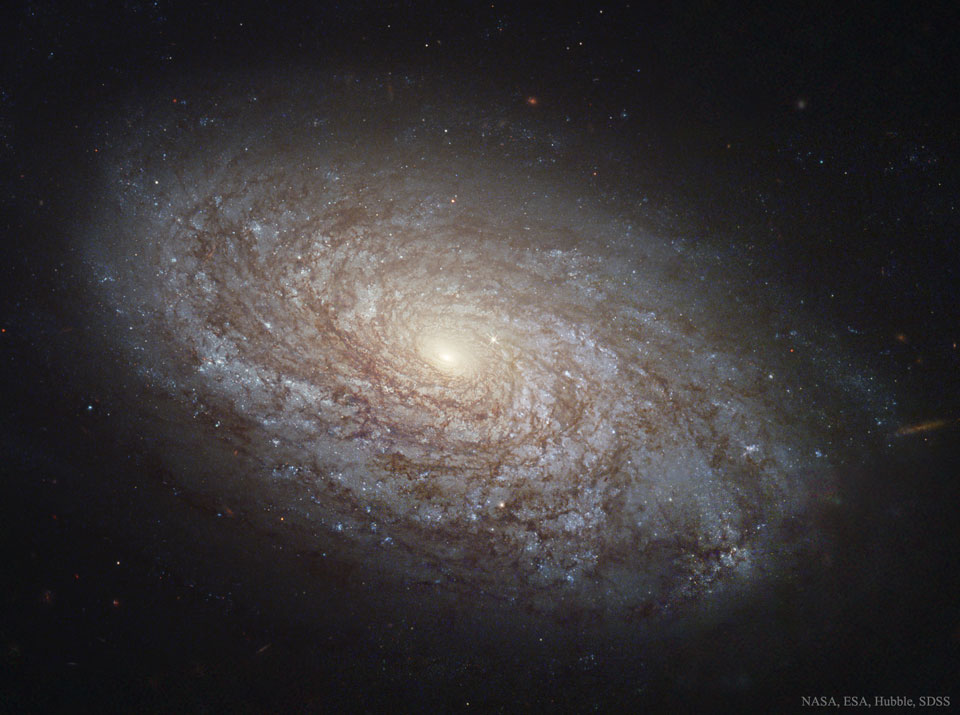
\includegraphics[width=0.7\linewidth]{Figures/NGC4414_modified}
			\caption{NGC4414 galaxy \todo{cite}}
		\end{figure}
	
		The dark matter halo used on the host, follows a NFW (Navarro–Frenk–White) profile, while the baryonic mass distribution of the galaxy depends on the redshift $z$. For high redshifts a gaseous disk with constant density followed by a density dependance with $r^{-2.2}$ is used, while for $z \approx 0$ a Hernquist model is applied \cite{choksi2017recoiling}.
		
	\subsection{Dark matter halo}
		For a dark matter halo following a NFW profile, the density at some distance $r$ is given by the formula:
		\begin{equation}\label{eq: dmdensity}
			\rho_\text{DM}(r) = \dfrac{\rho_0^\text{DM}}{\frac{r}{R_s}\left(1 + \frac{r}{R_s}\right)^2}
		\end{equation}
		
		Where $R_s$ and $\rho_0^\text{DM}$ are constants for a given dark matter halo. Using the density, the cumulative mass $M_\text{DM}(r)$ within some radius $r$ is given by the integral of the density over a volume, since \autoref{eq: dmdensity} is spherically symmetrical, the only dependance of the integral is with distance. On \autoref{eq: cumulativeDM} the $r'^2$ comes from the Jacobian of spherical coordinates, and the $4\pi$ from the solid angle.
		\begin{equation}\label{eq: cumulativeDM}
			M_{DM}(r) = \int\limits_0^{r} 4\pi {r'}^2\rho_\text{DM}(r')dr' = 4\pi\rho_0R_s^3\left[\ln\left(\dfrac{R_s + r}{R_s}\right) - \dfrac{r}{R_s + r}\right]
		\end{equation}
		
%		\begin{figure}[h]
%			\centering
%			\includegraphics[width=0.7\linewidth]{"../Files/Week 3/NFW_profile"}
%			\caption{Density and cumulative mass for a NFW profile with $\rho_0^\text{DM} = $ and $R_s = $.}
%		\end{figure}
		
		Since the mass of dark matter of a single galaxy diverges for $r \rightarrow \infty$ there is a radius called $R_\text{vir}$, at which the density of the NFW profile is 200 times the critical density $\rho_\text{crit}$, the minimum density for an expanding universe \todo{cite}.
		\begin{equation}
			R_\text{vir} = 200 \rho_\text{crit} = 200 \left(\dfrac{3H^2}{8\pi G}\right)
		\end{equation}
		
		Considering a concentration parameter $c(M_h, z)$ of dark matter in the halo, the following relation holds for the viral radius $R_\text{vir}$ and the scale radius $R_s$:
		\begin{equation}\label{eq: viralRadius}
			R_\text{vir} = c(M_h, z)R_s
		\end{equation}
		
		Where the concentration parameter, dependence with the dark matter halo mass and redshift is given by: 
		\begin{equation}
		c(M_h, z) = c_0(z)\left(\dfrac{M_h}{10^{13}M_\theta}\right)^{\alpha(z)}
		\end{equation}
		
		where $\alpha(z)$ and $c_0(z)$ were fitted using simulation data to the following functions \cite{choksi2017recoiling}:
		\begin{equation}
		c_0(z) = \dfrac{4.58}{2}\left[\left(\dfrac{1 + z}{2.24}\right)^{0.107} + \left(\dfrac{1 + z}{2.24}\right)^{-1.29}\right]
		\end{equation}
		
		\begin{equation}
		\alpha(z) = -0.0965 \exp\left(-\dfrac{z}{4.06}\right)
		\end{equation}
		
%		The relation of $R_\text{vir}$ with the concentration parameter is particularly useful to the simulation. As the system evolves on time, so does the viral radius due to the existing relation between time and redshift \cite{carmeli2006cosmic}.
%		\begin{equation}\label{eq: t_redshift}
%			t = \dfrac{2H^{-1}}{1 + (1 + z) ^ 2}
%		\end{equation}	
	
		\begin{figure}[h]
			\centering
			\includegraphics[width=0.7\linewidth]{"../Files/Week 3/darkmatter_concentration"}
			\caption{Dark matter concentration parameter as a function of the halo mass and the redshift.}
			\label{fig: dmconcentration}
		\end{figure}
	
		For a fixed halo mass, as time passes (smaller redshift), concentration of dark matter will increase, as can be shown on \autoref{fig: dmconcentration}. Because of \autoref{eq: viralRadius} the value of $R_\text{vir}$ will increase as well.
	
		\subsubsection{Baryonic profile}
			For high redshift the baryonic profile resembles that of a gaseous galaxy with a constant density for distances lower than $r_0 = 1\times10^{-3}$ kpc, followed by an $r^{-2.2}$ profile for greater distances as in \autoref{fig: baryonicprofilehigh}.
			
			\begin{equation}
				\rho_B(r) = \left \{
				\begin{matrix}
				\rho_0^B & \text{if $r < r_0$}\\
				\rho_0^B\left(\dfrac{r_0}{r}\right)^{2.2} & \text{if $r \geq r_0$}\\
				\end{matrix}
				\right.
			\end{equation}
			
			\begin{equation}
				M_B(r) = \left \{
				\begin{matrix}
				\dfrac{4}{3}\pi\rho_0^Br^3 & \text{if $r < r_0$}\\
				4\pi\rho_0^Br_0^{2.2} \left(r^{0.8} - r_0^{0.8}\right) + \dfrac{4}{3}\pi\rho_0^Br_0^3 & \text{if $r \geq r_0$} \\
				\end{matrix}
				\right.
			\end{equation}
			
			\pagebreak
		
			\begin{figure}[h]
				\centering
				\begin{subfigure}[b]{0.49\textwidth}
					\includegraphics[width=\textwidth]{"../Files/Week 3/gaseous"}
					\caption{Constant density profile for $r < 1$ pc, followed by a fall as $r^{-2.2}$ for $z \gg 0$.}
					\label{fig: baryonicprofilehigh}
				\end{subfigure}
				~ 
				\begin{subfigure}[b]{0.49\textwidth}
					\includegraphics[width=\textwidth]{"../Files/Week 3/hernquist"}
					\caption{Hernquist profile for mass distribution at $z \approx 0$.}
						\label{fig: baryonicprofilelow}
				\end{subfigure}
				\caption{Baryonic mass distributions for $z \gg 0$ and $z \approx 0$.}
				\label{fig: baryonicprofile}
			\end{figure}

		At low redshifts, stars have already been formed, and the baryonic profile is modeled as a Hernquist profile with half-mass radius $R_{1/2} = 0.01 R_\text{vir}$, as in \autoref{fig: baryonicprofilelow}. The half-mass radius, as the name implies, is the distance at which the cumulative mass is half the total mass \cite{hernquist1990analytical}.
		\begin{equation}
			\rho_B(r) = \dfrac{M_T^B \mathcal{R}_s}{2\pi r(r + \mathcal{R}_s)^3}
		\end{equation}
		\begin{equation}
			M_B(r) = \dfrac{M_T^B r^2}{(r + \mathcal{R}_s)^2}
		\end{equation}
		\begin{equation}
			R_{1/2} = \left(1 + \sqrt{2}\right)\mathcal{R}_s
		\end{equation}
		
	\subsection{Dynamical friction}
		As the black hole travels through the galaxy, dark matter, stars and gaseous materials from the medium interact with the black hole adding a drag force due to friction. Drag force is different in nature depending on it source, collisionless components, such as dark matter and stars, apply a drag force to the black hole that follows the standard Chandrasekhar formula \cite{choksi2017recoiling}.
		\begin{equation}
			a_\text{DF}^\text{DM}(r, v) = -4\pi G^2 M_\bullet\rho(r) \times \ln \Lambda\left(\erf{X} - \dfrac{2}{\sqrt{\pi}}Xe^{-X^2}\right)\dfrac{\vec{v}}{v^3}
		\end{equation}
		\begin{equation}
			X \equiv \dfrac{|v|}{\sqrt{2}\sigma_\text{DM}} \qquad \text{with } \sigma_\text{DM}(r) = \sqrt{\dfrac{GM_\text{DM}}{2R_\text{vir}}}
		\end{equation}
		
		 Gas on the other hand is collisional, special care must be taken since gas can cool behind a passing object, such as a black hole \cite{choksi2017recoiling}. A hybrid model for the drag force was proposed by Choksi, in which both subsonic and supersonic velocities are possible. To do so, a mach number was defined as:
		 \begin{equation}
			 \mathcal{M} \equiv \dfrac{v}{c_s}
		 \end{equation}
		 
		 where $v$ is the speed of the black hole, and $c_s$ is the local sound speed, which depends on local temperature, nevertheless it can be approximated to an isothermal halo as:
		 \begin{equation}
		 	c_s \approx 1.8(1 + z)^{1/2}\left(\dfrac{M_h}{10^7M_\odot}\right)^{1/3}\left(\dfrac{\Omega_M h^2}{0.14}\right)\text{ kms$^{-1}$}
		 \end{equation}
		 
		 where $\Omega_M$ and $h$ depend on the cosmology chosen. By knowing $\mathcal{M}$, the acceleration caused by gas can be written as:
		 \begin{equation}
		 	a^\text{gas}_\text{DF}(r, \vec{v}) = -4\pi G^2M_\bullet\rho_\text{gas}(r)\times f(\mathcal{M})\dfrac{\vec{v}}{v^3}
		 \end{equation}
		 
		 with
		 \begin{equation}
		 	f(\mathcal{M}) = \left\{
			\begin{matrix}
			0.5\ln\Lambda \left[\erf{\dfrac{\mathcal{M}}{\sqrt{2}}} - \sqrt{\dfrac{2}{\pi}}\mathcal{M}e^{-\mathcal{M}^2/2}\right]& \text{if $\mathcal{M} \leq 0.8$}\\
			1.5\ln\Lambda \left[\erf{\dfrac{\mathcal{M}}{\sqrt{2}}} - \sqrt{\dfrac{2}{\pi}}\mathcal{M}e^{-\mathcal{M}^2/2}\right] & \text{if $0.8 < \mathcal{M} \leq 1.7$}\\
			0.5\ln\left(1 - \mathcal{M}^{-2}\right) + \ln\Lambda & \text{if $\mathcal{M} > 1.7$}
			\end{matrix}
			\right.
		 \end{equation}
		 
		 finally, the gas density is taken as a power-law profile, $\rho_\text{gas}=\rho_0^\text{gas}r^{-n}$, were $1 \leq n \leq 3$ \cite{choksi2017recoiling}.
	
		\begin{table}[h]
			\centering
			\caption{Constants used in the simulation}
			\begin{tabular}{c|c}
				\hline
				\textbf{Constant} & \textbf{Value (unit)} \\
				\hline
				$n$ & 2\\
				$h$ & 0.678 \\
				$\Omega_M$ & 0.309 \\
				$\ln\Lambda$ & 2.3 \\
				$M_h$ & $1\times10^3$ ($10^5$\sm) \\
				$M_\bullet$ & 1 ($10^5$\sm) \\
				$M_T^B$ & 158 ($10^5$\sm) \\
				$R_s$ & 1.3 (kpc) \\
				$\mathcal{R}_s$ & 0.14 (kpc) \\
				$\rho_0^\text{DM}$ & 1700 ($10^5$\sm kpc$^{-3}$)\\
				$\rho_0^\text{gas}$ & 0.01 ($10^5$\sm kpc$^{-3}$)\\
				\hline
			\end{tabular}
		\end{table}
	
%\section{Metodología}
%	El paso inicial consiste en generar un cuerpo con $10^8$ \sm usando la librer\'ia REBOUND, el cual tendr\'a la siguiente ecuaci\'on de movimiento:
%	\begin{equation}
%		\ddot{\vec{x}} = \left(-\dfrac{GM_h(x)}{x^2} + a_{DF}-\ddot{x}\dfrac{\dot{M_\bullet}}{M_\bullet} -qH^2x\right)\hat{x}
%	\end{equation}
	
%	donde $M_h$ corresponde con la masa del halo de la galaxia, $a_{DF}$ con la aceleraci\'on debida a la fricci\'on din\'amica, la cual se modela usando la f\'ormula de Chandrasekhar para la materia oscura y el modelo h\'ibrido descrito por Choksi para la materia visible \cite{choksi2017recoiling}. El tercer t\'ermino tiene en cuenta la acreci\'on de masa por el agujero negro, y el \'ultimo la aceleraci\'on cosmol\'ogica.
%	
%	Dicha ecuaci\'on ser\'a integrada usando un esquema \textit{Leapfrog}, el cual se encuentra implementado en la librer\'ia REBOUND. Usando como condiciones iniciales $\vec{x} = (0,0,0)$ km y $\dot{\vec{x}} = (70, 0, 0)$ km$s^{-1}$, e intervalos de integraci\'on temporales de 1000 años, se busca reproducir los comportamientos observados por Choksi y colaboradores, para comprobar que el algoritmo implementado funcione de manera adecuada.
%	
%	Posteriormente ser\'an introducidas las modificaciones al potencial cambiando $M_h(x)$ por $M_h(x, y, z)$, donde los pesos de cada dimensi\'on ser\'an determinados de manera aleatoria para cada simulaci\'on. Al mismo tiempo se asignar\'an velocidades iniciales aleatorias, logar\'itmicamente espaciadas en el rango de 0 kms$^{-1}$ hasta 3000 kms$^{-1}$, sin ninguna direcci\'on preferente. Para cada sistema generado se realizar\'a la evoluci\'on en el tiempo usando integradores num\'ericos distintos. El tiempo aproximado de cada simulaci\'on se encuentra en el orden de 100$^6$ a\~nos, por lo cual ser\'an necesarias cerca de cien mil interaciones por cada conjunto de par\'ametros escogidos.
%	
%	Las simulaciones ser\'an realizadas en el cluster de la universidad (HPC) con el fin de paralelizar procesos, minimizando el tiempo de simulación y de esta forma lograr la mayor cantidad de simulaciones posibles, con el fin de obtener una cantidad significativa de datos de validación. A partir de estos, se obtendr\'an las distribuciones de probabilidad de los tiempos de retorno, y la cuantificaci\'on de la caoticidad de la trayectoria.